\documentclass[paper=a4, USenglish, numbers=noenddot]{scrartcl}
\usepackage[utf8]{inputenc}
\usepackage[T1]{fontenc}
\usepackage{amsmath}
\usepackage{amssymb}
\usepackage{tikz}
\usetikzlibrary{matrix,arrows,patterns,intersections,calc,decorations.pathmorphing}

\begin{document}

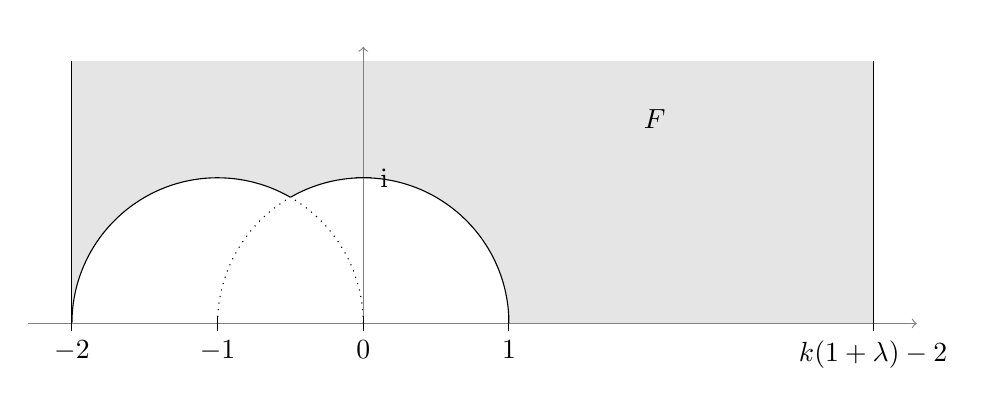
\begin{tikzpicture}[scale=1.85]
   \fill[gray!20!white] (-2,0) arc (180:60:1) arc (120:0:1) (3.5,0) -- (3.5,1.8) -- (-2,1.8) -- (-2,0);
   
   \draw (-2,0) -- (-2,1.8);
   \draw (3.5,0) -- (3.5,1.8);
   
   \draw (-2,0) arc (180:60:1);
   \draw[dotted] (0,0) arc (0:60:1);
   \draw (1,0) arc (0:120:1);
   \draw[dotted] (-1,0) arc (180:120:1);

   \draw[->, gray] (-2.3,0) -- (3.8,0) node[right] {};
   \draw[->, gray] (0,0) -- (0,1.9) node[above] {};		% Koordinatenachsen

   \draw (-2,0.05) -- (-2,-0.05) node[below] {$-2$};
   \draw (-1,0.05) -- (-1,-0.05) node[below] {$-1$};		
   \draw (0,0.05) -- (0,-0.05) node[below] {$0$};
   \draw (1,0.05) -- (1,-0.05) node[below] {$1$};
   \draw (3.5,0.05) -- (3.5,-0.05) node[below] {$k(1+\lambda)-2$};
   \draw (-0.05,1) -- (0.05,1) node[right] {$\mathrm{i}$};				% Achsenbeschriftung
   
   \draw (2,1.4) node {$F$};
  \end{tikzpicture}

\end{document}